\chapter{GRAPHPLAN}
\thispagestyle{chapterBeginStyle}

\section{Wprowadzenie}
    \textbf{GRAPHPLAN} jest algorytmem do planowania akcji działający w dziedzinie zdefiniowanej
    przez język STRIPS, dodatkowo bazuje na paradygmacie, który autorzy algorytmu określają jako "graf planujący" \cite{GRAPHPLAN}.
    \begin{figure}[H]
        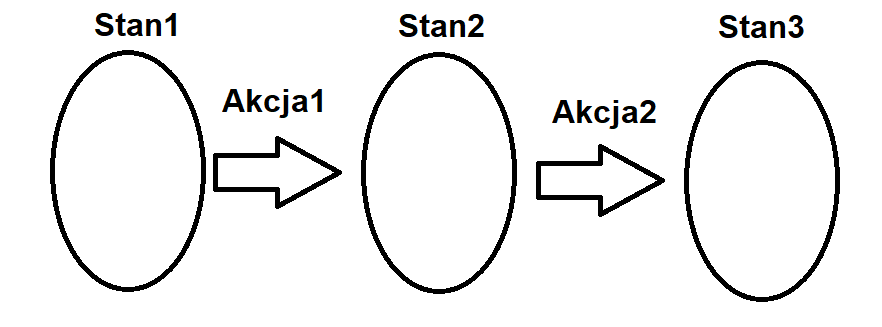
\includegraphics[scale=0.5]{PlanningGraph}
        \centering
        \caption{Najogólniejsza forma grafu planującego. Składa się on z węzłów, zwanych stanami oraz krawędzi zwanych akcjami. Docelowo poszczególne 
        stany oraz akcje są parami różne, jednak mogą zajść sytuacje, gdy powtórzenie któregoś z komponentów będzie wymagane do uzyskania odpowiedniego
        celu.}
        \label{PlanningGraph}
    \end{figure}
    Pierwotną ideę grafu planującego przedstawiono na obrazku \ref{PlanningGraph}. W trakcie dalszego omawiania metodologii GRAPHPLAN powyższa 
    rycina będzie pojawiała się ponownie z coraz to większym poziomiem szczegółowości.
    Ze względu na fakt, iż Graphplan opiera się na języku STRIPS musi mieć jasno zdefiniowane: stan początkowy, akcje oraz cel, który pragniemy uzyskać.
    Dzięki swojej strukturze Graphplan w swojej naturze podobny jest do programowania dynamicznego.

\section{Warunki początkowe}
    \begin{definition}
        \label{ZasadaSwiata}
        \textbf{Zasada zamkniętego świata} - Zasada, wedle której pojęcia, które nie są ściśle opisane w świecie są nieprawdziwe.
    \end{definition}
    GRAPHPLAN, w odróżnieniu od człowieka, musi być w posiadaniu całej wiedzy o świecie, aby móc rozpocząć działanie. Przez całą wiedzę o świecie rozumie się
    posiadanie informacji na temat każdego obiektu oraz jego stanu. Wiąże się to ściśle z faktem,
    iż GRAPHPLAN operuje zgodnie z definicją \ref{ZasadaSwiata}. 
    Przed dalszą częścią pracy należy dokonać pewnego wyróżnienia. Słowo \textbf{stan} pojawia się w dwóch znaczeniach:
    stan jako pojedyncza informacja o obiekcie w świecie (Przykład: klocek B na stole numer 3) oraz stan, jako zbiór wszystkich takich informacji w danym momencie czasu.
    Z tego względu wprowadzono nowe pojęcie- "Poziom stanów", które należy stosować jako oznaczenie wszystkich informacji o świecie w danym momencie.
    \begin{definition}
        \label{PoziomStanow}
        \textbf{Poziom stanów} - Zbiór informacji o stanach wszystkich obiektów w świecie w danej jednostce czasu \textit{t}
    \end{definition}
    Szczególnym poziomem stanów jest poziom oznaczany jako pierwszy i nazywany \textbf{Warunkami początkowymi}, którego poprawne zdefiniowanie jest kluczowym aspektem w kontekscie
    uzyskania poprawnego wyniku przez algorytm.
    Analizując ponownie przykład \ref{Przyklad1} mylnym jest myśleć, iż jedyną informacją, jaką algorytm powinien posiadać o świecie jest pobyt klocka A na lewej platformie. Również
    istotną informacją jest brak klocka na platformie prawej, czyli informacja, ze jest on \textit{pusty}. Mimo poczucia nadmiarowości tej informacji, w dalszej części pracy wyjaśni
    się, dlaczego ta informacja jest niezbędna do uzyskania poprawnego wyniku.
    Przykład świata przedstawionego oraz skonstruowanego dla niego stanu początkowego:
    \begin{figure}[H]
        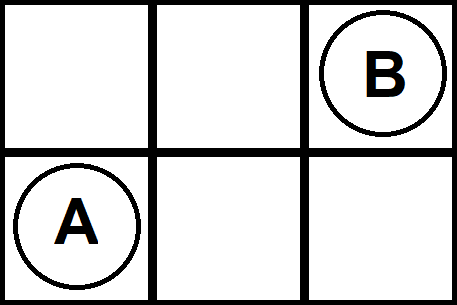
\includegraphics[scale=0.5]{PrzykladSP}
        \centering
        \caption{Przykładowy moment startowy przyszłego planu. Za pomocą okręgów oznaczono roboty, natomiast poprzez kwadraty oznaczone są kafelki- miejsca,
        po których mogą poruszać się roboty.}
        \label{PrzykladSP}
    \end{figure}
    Na powyższym przkładzie, zgodnie z ideą Graphplanu wyszczególniamy 6 stanów początkowych. Dodatkowo należy doprecyzować pojęcie bycia robota na danym kafelku. Wykonano to 
    przy pomocy dwuargumentowej relacji \textit{na}, która jako pierwszy argument przyjmuje sygnaturę robota, a na drugim- numer kafelka. Na potrzeby przykładu ustalono, iż 
    numerowanie odbywa się rzędami od lewej do prawej. Zgodnie z tymi ustaleniami pozycję robotów A i B możemy określić w następujący sposób: \textit{$na(A,4)$} oraz 
    \textit{$na(B,3)$}. Również pustość kafelków należy sformalizować wprowadzając relację jednoargumentową o nazwie \textit{pusty}, która przyjmuje jako argument numer
    pustego kafelka. Reasumując, zbiorem stanów początkowy dla analizowanego przykładu \ref{PrzykladSP} jest: 
    \begin{equation}
        \{pusty(1),pusty(2),na(B,3),na(A,4),pusty(5),pusty(6)\}
        \label{ZbiorPoczatkowy}
    \end{equation}
\section{Akcje}
    Posiadając dobrze określony stan początkowy następnym krokiem będzie zdefiniowanie akcji. Zgodnie z \ref{Akcje} oraz wzmiance o akcjach w planerze STRIPS,
    akcja musi składać się z trzech komponentów:
    \begin{itemize}
        \item Czynności
        \item Warunków zajścia
        \item Efektów zajścia
    \end{itemize}
    Z tego powodu każdą z akcji będziemy traktować jako trójkę 
    \begin{equation}
        A=(C,W,E)
    \end{equation}
    gdzie każda z liter odpowiada pierwszej literze wyżej wymienionego pojęcia. 
    W skład efektów wchodzą dwa pojęcia wprost z terminologii STRIPS- dodające i usuwające. Dzięki takiemu podziałowi łatwiejszym będzie 
    zachowanie silnego podziału między przyczynami a efektami akcji. 
    Jedyną czynnością, którą należy brać pod uwagę w ramach \ref{PrzykladSP} jest czynność \textit{ruch}, którą definiujemy jako trzyargumentową relację:
    \begin{equation}
        ruch(R,S,D)
    \end{equation}
    , gdzie R odpowiada robotowi, który musi się przemieścić z kafelka oznaczonego literą S (kafelek startowy) na kafelek oznaczony
    literą D (kafelek docelowy).
    
    Następnymi składowymi są odpowiednio \textit{Warunki} jak i \textit{Efekty}. Warunki traktujemy jako zbiór wszystkich stanów, które muszą być 
    prawdziwe w danej jednostce czasu. Jeśli choć jeden stan nie jest spełnialny, opisywana akcja nie może zostać wykonana w danym ruchu.
    Efekty natomiast definiujemy jako następującą parę:
    \begin{equation}
        E=(D,U)
    \end{equation}
    gdzie D oznacza efekty dodające, a U- efekty usuwające.
    \begin{figure}[H]
        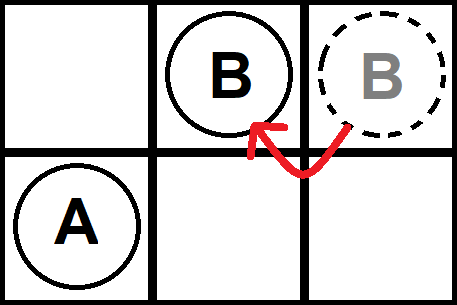
\includegraphics[scale=0.5]{PrzykladRuch}
        \centering
        \caption{Obrazowe przedstawienie ruchu robota B z kafelka 3 na kafelek 2}
        \label{PrzykladRuch}
    \end{figure}
    Niech rozpatrywaną akcją będzie przemieszczenie robota B z pozycji 3 na pozycję 2,
    przedstawiona na \ref{PrzykladRuch}. Biorąc pod uwagę, iż stanem początkowym jest \ref{ZbiorPoczatkowy} Warunkami zajścia zdarzenia
    będą: $na(R,S)$ oraz $pusty(D)$. Dla efektów natomiast sytuacja wygląda następująco: efektami dodającymi są $na(R,D)$ oraz $pusty(S)$, które informują o tym, iż klocek 
    wykonał ruch z kafelka S na kafelek D, a efektami usuwającymi $\sim na(R,S)$ oraz $\sim pusty(D)$, które informują o tym, iż kafelek S został zwolniony, 
    oraz robot nie znajduje się już na kafelku S. Przy pomocy matematycznego symbolu negacji wyrażono nieprawdziwość danego stanu.

        Posiadająć następującą wiedzę poniżej zdefiniowano jedyną akcję znajdująca się w prezentowanym przykładzie:
    \begin{equation}
        \label{Ruch}
        A=(ruch(R,S,D),\{na(R,S),pusty(D)\},\{na(R,D),pusty(S),\sim na(R,S),\sim pusty(D)\})
    \end{equation}
    Podstawiając za $R=B$, $S=3$, a $D=2$ otrzymujemy następującą akcję:
    \begin{equation}
        A=(ruch(B,3,2),\{na(B,3),pusty(2)\},\{na(B,2),pusty(3),\sim na(B,3),\sim pusty(2)\})
    \end{equation}
    
    Analogicznie można zdefiniować ruch na kafelek numer 6, oraz dwa ruchy dla robota o sygnaturze A.


    \subsection{Typy akcji}
    Definicja \ref{ZasadaSwiata} znajduje również swoje odzwierciedlenie w akcjach. Niech rozpatrywanym przykładem będzie wciąż przykład \ref{PrzykladSP}.
    W pierwszym kroku wykonano akcję $ruch(B,3,2)$.Z persepktywy człowieka jest to wystarczająca informacja, aby móc wydedukować, co we wskazanym etapie
    generowania planu  dzieje się z robotem \textbf{A}. Otóż robot A w pierwszym ruchu zostaje na tym samym kafelku. 
    Jednakże ze względu na zamkniętość świata 
    algorytmu należy go również poinformować go o tym, w jakim stanie po pierwszym kroku ma znajdować się robot A. Wykonywane jest to przy pomocy 
    akcji, zwanych \textbf{akcjami potrzymującymi}.
    \begin{definition}
        \label{Persist}
        \textbf{Akcja podtrzymująca} - Akcja, która przenosi stan obiektu w czasie $t$ nienaruszonym do poziomu stanów w czasie $t+1$
    \end{definition}
    Akcjami podtrzymującymi należy również informować świat o stanach kafelków, które nie brały udziału w akcji robota B. Przykładem takiego jest 
    kafelek 1, który w stanie początkowym, jak i w stanie następnym ciągle zachowuje swój stan jako pusty. Akcje podtrzymujące oznaczono 
    słowem kluczowym \textbf{zostań}
    Ponadto akcja typu \textit{ruch}, które aktywnie zmienia stan świata w dalszej części pracy otrzyma miano \textbf{akcji aktywnej}.
    \begin{definition}
        \label{Active}
        \textbf{Akcja aktywa} - Akcja, która zmienia stan obiektu między stanami w czasie $t$ i $t+1$.
    \end{definition}

    Posiadając powyższy podział akcji poniżej przedstawiono pełen zbiór akcji w pierwszym kroku algorytmu. Wartym odnotowania jest, iż ze względów
    estetycznych podawawnie akcji podtrzymujących będzie często pomijane, jednakże nie można zapomnieć o ich występowaniu oraz o ich kluczowej roli 
    w generowaniu precyzyjnego planu.
    \begin{align*}
        Akcje &= \{zostan(pusty(1)),zostan(pusty(2)),zostan(pusty(5)),zostan(pusty(6)),zostan(na(B,3)), \\
        &zostan(na(A,4)),ruch(B,3,2),ruch(B,3,6),
        ruch(A,4,1),ruch(A,4,5)\}
    \end{align*}
    Należy również nadmienić, iż podobnie jak w stanach, dla akcji wprowadza się pojęcie \textbf{Stanu akcji}, które funkcjonuje jako zbiór 
    składający się ze wszystkich możliwych akcji do wykonania w danej jednostce czasu.
    \begin{figure}[H]
        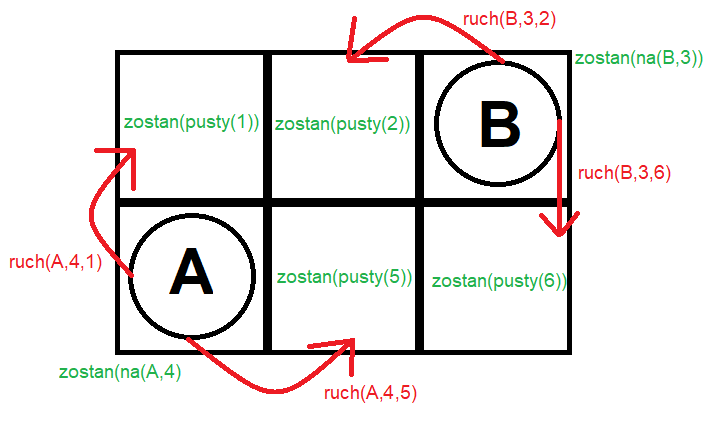
\includegraphics[scale=0.5]{PrzykladAkcje}
        \centering
        \caption{Obrazowe przedstawienie wszystkich akcji w pierwszym kroku algorytmu, akcje opisane przy użyciu czcionki o kolorze zielonym 
        symbolizują akcje podtrzymujące, natomiast o kolorze czerwonym- akcje aktywne}
        \label{PrzykladAkcje}
    \end{figure}
    

\section{Definiowanie świata}
    Zdecydowanie najtrudniejszym aspektem modelowania świata jest dokładne przedstawienie wszystkich zależności, jakie algorytm musi znać,
    aby mógł bezbłędnie wnioskować w prezentowanej przestrzeni. Analizując przykład \ref{PrzykladSP} dokonano przedstawienia schematu 
    generowania poziomu stanów początkowych oraz poziomu akcji. Zadając pytanie algorytmowi \textit{Jakie działania należy podjąć, aby jak najszybciej
    przesunąć robota A z klocka 4 na klocek 6} algorytm odpowie w następujący sposób: $ruch(A,4,6)$, jednakże przyglądając się uważnie przedstawionemu światu 
    zauważono, iż taki plan byłby realny jedynie, gdyby akcja $ruch$ oznaczała latanie- wtedy faktem jest, iż istnieje możliwość pominięcia kafelka 5 podczas 
    przemieszczenia. Niespójnośc ta pojawiła się z faktu, iż w żadnym momencie nie określono w jaki sposób dokładnie funkcjonuje czynnośc oznaczona jako \textit{ruch}.
    Wedle definicji \ref{Ruch} wszystkie warunki, aby robot mógł przemieścić się z kafelka 4 na 6 zostały spełnione.

    Naprawić ten problem można przy pomocy uściślenia wykonywanej czynności. Do tego potrzebne będzie wprowadzenie relacji \textit{sąsiad}, która 
    przyjmuje dwa argumenty- numery kafelków, które ze sobą sąsiadują. Zakładając, iż sąsiadujące kafelki to takie, które mają wspólną ścianę, sąsiadami 
    kafelka 1 są kafelki: 2 oraz 4. Dla pozostałych przestrzeni dokonano analogicznego wygenerowania listy sąsiadów. Dzięki tej operacji, 
    akcję ruch zdefiniowano w następujący sposób:
    \begin{equation}
        ruch(R,S,D) \textnormal{:-} sasiad(S,D)
    \end{equation}
    Czynność ruchu w powyższym przypadku została określona zgodnie z semantyką języka programowania \textbf{PROLOG}. Należy to rozumieć w następujący sposób:
    po lewej stronie znaku \textbf{:-} znajduje się \textit{konkluzja}, natomiast po prawej- \textit{przesłanka}. Naturalnym odczytem przedstawionej sytuacji
    będzie zdanie \textit{"Jeśli kafelki S i D są sąsiadami to możliwym do wykonania jest ruch między tymi kafelkami"}
    \begin{figure}[H]
        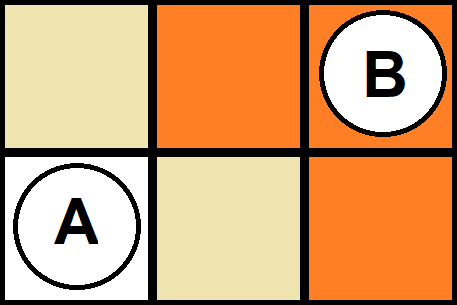
\includegraphics[scale=0.5]{PrzykladSasiad}
        \centering
        \caption{Graficzne przedstawienie relacji sąsiedztwa dla kafelka numer 4. Kolorem kremowym oznaczono miejsca, z którymi sąsiaduje, natomiast 
        pomarańczowym- te, z którymi nie sąsiaduje. Oznacza to, iż do kafelków pomarańczowych nie można dostać się wykonując jeden ruch}
        \label{PrzykladAkcje}
    \end{figure}
    Taka definicja ruchu pozwala w skuteczny sposób oddać intuicję, która wynika z poglądowego obrazka przedstawiającego rozpatrywany świat.
    Niewystarczającym jest określenie relacji $sasiad(1,2)$, gdyż wedle tego faktu kafelek pierwszy sąsiaduje z kafelkiem drugim, jednakże nie oznacza 
    to, iż kafelek drugi sąsiaduje z kafelkiem pierwszym. Z tego dla każdej pary kafelków A i B do zbioru sąsiadów należy dodać dwie relacje:
    $sasiad(A,B)$ oraz $sasiad(B,A)$. Inna sytuacja byłaby, gdyby ruch był możliwy jedynie w jedną stronę, jednakże tutaj taki stan rzeczy nie występuje.


    Oprócz definicji sąsiedztwa należy również zabezpieczyć się przed sytuacją, gdy dwa roboty będą chciały w tym samym momencie znaleźć się na tym samym 
    kafelku. Dodatkowo kafelek A nie może znajdować się w dwóch stanach jednocześnie: $pusty(A)$ oraz $na(R,A)$, gdzie R oznacza dowolnego robota. 
    Wymodelowanie tych ograniczeń jest prostym, lecz istotnym zadaniem implementując przedstawianą metodologię, które zostanie poruszone w ramach 
    przedstawiania pojęcia "wzajemnego wykluczania".
    
    
    Odpowiednie wymodelowanie świata wedle wzorców języka STRIPS może wydawać się trudnym oraz żmudnym zajęciem, jednakże przebrnąwszy 
    przez ten etap algorytm jest zwarty i gotowy do generowania planów dla wprowadzonych celów.


\section{Warstwy grafu}
    Składowe planu grafującego można podzielić na dwa typy: jeden, wyszczególniony jako poziomy stanów oraz drugi- poziomy akcji. Aby lepiej 
    uwidocznić zależność poziomu akcji od warunków początkowych oraz zależność kolejnego poziomu stanów od efektów akcji graf planujący 
    z \ref{PlanningGraph} ulegnie lekkiej modyfikacji. 
    \begin{figure}[H]
        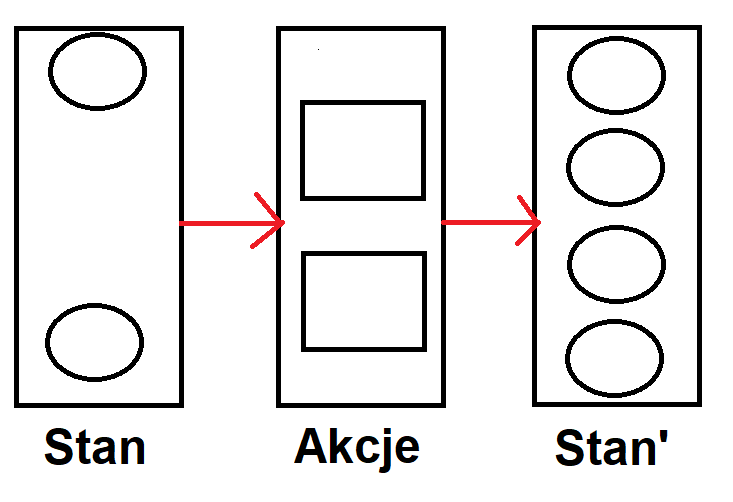
\includegraphics[scale=0.5]{PlanningGraphStates}
        \centering
        \caption{Modyfikacja do grafu planującego wprowadzona w poprzednich podrozdziałach. Wprowadzono zależności akcji od stanu poprzedniego, oraz stanu 
        następnego od akcji.}
        \label{PlanningGraphStates}
    \end{figure}
    Następnym krokiem będzie wprowadzenie definicji \textbf{Warstwy grafu}
    \begin{definition}
        \label{Warstwa}
        \textbf{Warstwą} - grafu nazywamy połączenie poziomu stanów oraz wynikającego z niego poziomu akcji
    \end{definition}
    Przez $i$-tą warstwę grafu oznaczono stan świata w $i$-tym momencie czasu. Ze względu na charakterystykę planera czas traktowany jest w sposób dyskretny-
    każda ze zdefiniowanych akcji zajmuje zawsze tyle samo czasu oraz zawsze kończy się tym samym efektem. Poziomy stanów jak i poziomy akcji 
    należące do tej samej $i$-tej warstwy nazywamy poprzez dołączenie do ich nazwy numera, odpowiadającego obecnej iteracji algorytmu
    iteracji algorytmu.
    \begin{figure}[H]
        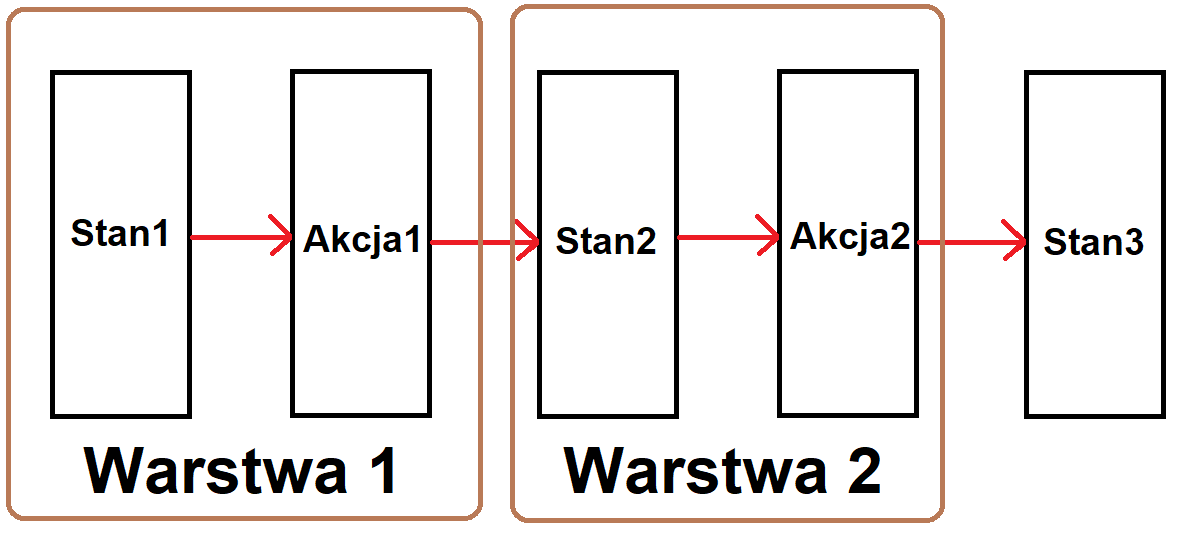
\includegraphics[scale=0.5]{PlanningGraphLevels}
        \centering
        \caption{Przedstawienie sposobu wyznaczania warstw w algorytmie planującym. Poziom stanów oraz akcji wchodzący w skład danej warstwy 
        wyróżniony jest poprzez konkatenację nazwy oraz liczby symbolizującej numer warstwy.}
        \label{PlanningGraphLevels}
    \end{figure}
    Dzięki wprowadzeniu definicji warstwy po wygenerowaniu 
    planu natychmiast wiadomo ile kroków należy wykonać, a co za tym idzie- ile czasu należy poświęcić, aby osiągnąć ustalony cel. 

    \section{Równoległość}
    W poprzednich paragrafach na pojedynczym poziomie akcji rozpatrywano conajwyżej jedną akcję aktywną, jednakże główną siła GRAPHPLANU, jest 
    możliwość jego reprezentacji jako częściowego porządku. To pozwala w prosty sposób wprowadzić pojęcie równoległości między akcjami. 
    \begin{definition}
        \label{Warstwa}
        Dwie (lub więcej) akcje  mogą zostać wykonane \textbf{równolegle}, gdy po ich wykonaniu w tej samej warstwie $i$, warstwa $i+1$ nie będzie 
        zawierała w sobie żadnych sprzeczności.
    \end{definition}
    Przyglądając się rysunkowi \ref{PrzykladSP} od razu należy zauważyć, iż w stanie początkowym ruch robota A nie wpływa w żaden sposób na otoczenie
    robota B. Z tego względu dwie przykładowe akcje $ruch(A,4,5)$ oraz $ruch(B,3,2)$ wręcz należy wykonać w tej samej jednostce czasu, czyli w pierwszym
    poziomie akcji. 
    \begin{figure}[H]
        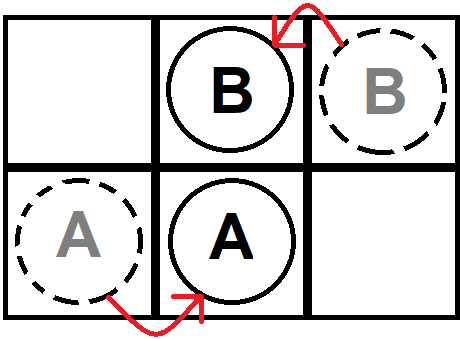
\includegraphics[scale=0.5]{PrzykladRownolegle}
        \centering
        \caption{Przykład możliwości zastosowania równoległości w planowaniu działania. Należy zauważyć, iż ruchy robotów w żaden sposób ze sobą
        nie kolidują.}
        \label{PrzykladRownolegle}
    \end{figure}
    
    Po wprowadzeniu definicji równoległości, również definicja kroku musi ulec ewolucji. 
    \begin{definition}
        \label{Krok}
        \textbf{Krokiem} algorytmu nazywamy zbiór wszystkich możliwych do realizacji akcji w danej warstwie.
    \end{definition}
    Dzięki naniesionej poprawce pozbywamy się łatki mówiącej o tym, iż pojedyncza zmiana stanu jest ściśle związana z jedną akcją.W tym miejscu należy 
    zauważyć, iż poprzednie analizy zawierały spore uproszczenie, gdyż akcje podtrzymujące również należą do kroku algorytmu, co zostało zaprezentowane
    w trakcie kreowania pierwszej warstwy akcji dla rozpatrywanego przykładu. 

    Istnieją przypadki, gdy podmiot realizujący plan nie jest w stanie wykorzystać benefitów płynących z możliwości dokonywania akcji równolegle, 
    na przykład ze względu na ograniczone zasoby. GRAPHPLAN również rozwiązuje ten problem, pozwalając przekształcać swój częsciowy porządek 
    na porządek liniowy w dość dowolny sposób. Otóż akcje z danej warstwy mogą być wykonywane w dowolnej kolejności, gdyż w żaden sposób ze sobą nie 
    kolidują. Z persepktywy algorytmu najważniejszym jest, aby stan świata $i$ i $i+1$ był zgodny z informacjami jakie posiada o świecie. Zgodnie z
    przykładem \ref{PrzykladRownolegle} widać, iż to, czy akcja $ruch(A,4,5)$ zostanie wykonana przed akcją $ruch(B,3,2)$ lub to, czy akcja 
    $ruch(B,3,2)$ odbędzie się prxed $ruch(A,4,5)$- efekt końcowy jest identyczny.

    \subsection{Wzajemne wykluczanie}
    Twórcy algorytmy wprowadzając równoleglość, zdawali sobie sprawę z mocy tego podejścia. Dzięki temu ogromna liczba planów ulega redukcji
    jeśli chodzi o wymagany czas wykonania. Jednakże równoległość wprowadza kolejny istotny problem w prezentowanym świecie, a mianowicie- co, gdy
    wykonanie dwóch akcji będzie wprowadzało sprzeczność w następnym poziomie świata? Sytuacja ta została przedstawiona na poniższym rysunku
    \begin{figure}[H]
        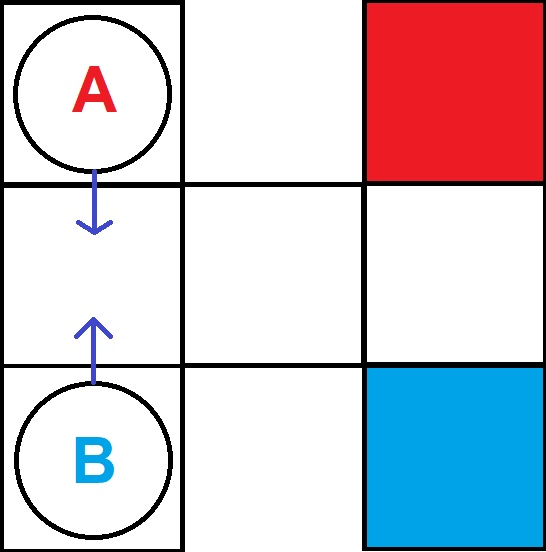
\includegraphics[scale=0.5]{PrzykladRownolegleZle}
        \centering
        \caption{Przykład świata, w którym wprowadzenie równoległości dla pierwszej warstwy algorytmu. Dwa roboty próbują przenieść się na ten sam kafelek
        w tej samej jednostce czasu. Odpowiednio kolorami:
        czerwnoym i niebieskim oznaczono roboty, oraz kafelki, które są ich celem.}
        \label{PrzykladRownolegle}
    \end{figure}
    
    Zmusiło to twórców algorytmu do wporwadzenia pojęcia \textbf{relacji wykluczania}. 
    O akcjach wzajemnie się wykluczających (ang. actions mutually exclusive) wspomiano w ramach definiowana świata. Pojęcie ów można 
    określić w następujący sposób:
    \begin{definition}
        \label{Warstwa}
        \textbf{Relacją wzajemnie wykluczającą się} - jest relacją między akcjami(stanami), która informuje o tym, iż nie istnieje plan taki,
        aby dwie wybrane akcje(stany) mogły być prawdziwe w tej samej jednostce czasu $t$
    \end{definition}
    Przykładem stanów wykluczających jest para: $pusty(1)$ oraz $\sim pusty(1)$. Kafelek nie może być pusty jak i niepusty jednocześnie.
    Przykład dwóch akcji wykluczających przedstawiono na rysunku \ref{PrzykladRownolegle}. Należy zauważyć, iż wzajemne wykluczanie się 
    jest rozpatrywane na poziomie jednej warstwy- brak możliwości wykonania dwóch akcji w warstwie $i$ nie przenosi się automatycznie na 
    warstwę $i+1$. Świat może zostać na tyle przeobrażony, iż ich wspólna egzystencja nie spowoduje wprowadzenia niezgodności.
    Kolejnym naturalnym krokiem jest ustalenie, kiedy akcje oraz stany są ze sobą w relacji wykluczającej. 
    \subsubsection{Wykluczanie się akcji}
    Dwie akcje mogą być ze sobą w relacji wzajemnie wykluczającej w trzech następujących przypadkach:
    \begin{enumerate}
        \item Niespójny efekt- przypadek, w którym zbiór efektów jednej z akcji 
        jest negowany przez zbiór efektu drugiej
        \item Przeszkadzanie - przypadek, w którym jedna z akcji usuwa warunki 
        zajścia akcji drugiej 
        \item Konkurencyjne potrzeby- przypadek, w którym warunki zajścia akcji 
        są ze sobą w relacji wykluczającej.
    \end{enumerate}
    Poniższe przykłady w obrazowy sposób przedstawiają każdy w wyżej wymienionych
    przypadków:


    \subsubsection{Wykluczanie się stanów}
    Dwa stany są ze sobą w relacji wzajemnie wykluczającej w dwóch następujacych przypadkach:
    \begin{enumerate}
        \item Negacja- przypadek, w którym jeden ze stanów jest negacją drugiego
        \item Niespójne powstanie- wszystkie akcje z poprzedniej warstwy, które prowadza 
        do utworzenia ów stanów są ze sobą w relacji wykluczającej
    \end{enumerate}
\section{Wyszukiwanie planu}

\section{Prosty przykład}
